\documentclass{article}

\usepackage{mathtools,amsfonts}
\usepackage{enumerate}
\usepackage{fullpage}
\usepackage{array}
\usepackage{fancyvrb}

\begin{document}
\thispagestyle{empty}

\begin{center}
  \textbf{\Large Beginner Test 1}
  % LEVEL is Senior, Intermediate or Beginner
  % NUMBER is the test number: 1, 2, etc.
  \\ \vspace{1em}
  \textbf{\large January Camp 2021}
  \\ \vspace{1em}
  \textbf{\large Time: $2\frac{1}{2}$ hours}
\end{center}

\vspace{24pt}

\begin{enumerate}[1.]


\item What is the ratio of the areas of the two squares given below:
	\begin{center}
	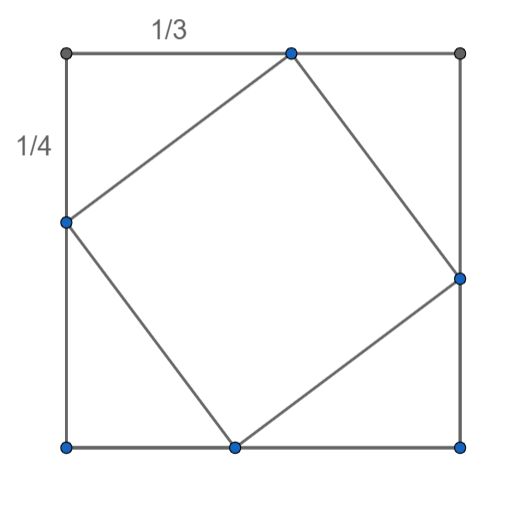
\includegraphics[scale=0.4]{beginner_test_1_img_2.png}	
	\end{center}
Remember to prove your answer.
% Tim


\item Find, with proof, the smallest three different positive integers whose squares sum to the square of an integer. % Tim


\item Find, with proof, 4 fractions strictly between $\frac{1}{3}$ and $\frac{1}{2}$ with denominator less than 10. % Tim


\item What fraction of the following shape is shaded:
	\begin{center}
	
\includegraphics[scale=1.0]{beginner_test_1_img_1.png}	
	\end{center}
Prove your answer.\\
\textit{Note: The dots are spaced evenly around the circle and the only interior point used is the center of the circle.}
% Catriona Shearer, https://mathwithbaddrawings.com/2018/10/03/twenty-questions-of-maddening-delicious-geometry/


\item You are given that T,W,O,N,E are all different digits from 1 to 9 such that T+O+N=6 and:
\begin{center}
\begin{tabular}{m{1cm} m{0.5cm} m{0.5cm} m{0.5cm}}
&T&E&N\\
+&T&W&O\\
\hline
&O&N&E\\
\hline
\end{tabular}
\end{center}
Find, with proof, the values of T,W,O,N,E.
% Tim


\item Ralph and Phil are playing a game. They have R12 in a bank account and can only withdraw coins of values R1, R2 and R5. The winner is the player who withdraws the last coin. If Ralph starts and they then alternate withdrawing one coin each (with a value of their choice), who has the winning strategy and how can they win?\\
\textit{Note: A winning strategy must be able to beat any sequence of moves that the opposing player decides to make.}


\item You are given the following shape: % South Africa, Tim's Assorted Combinatorics Questions 2020, Q2 (7 marks)
	\begin{center}
	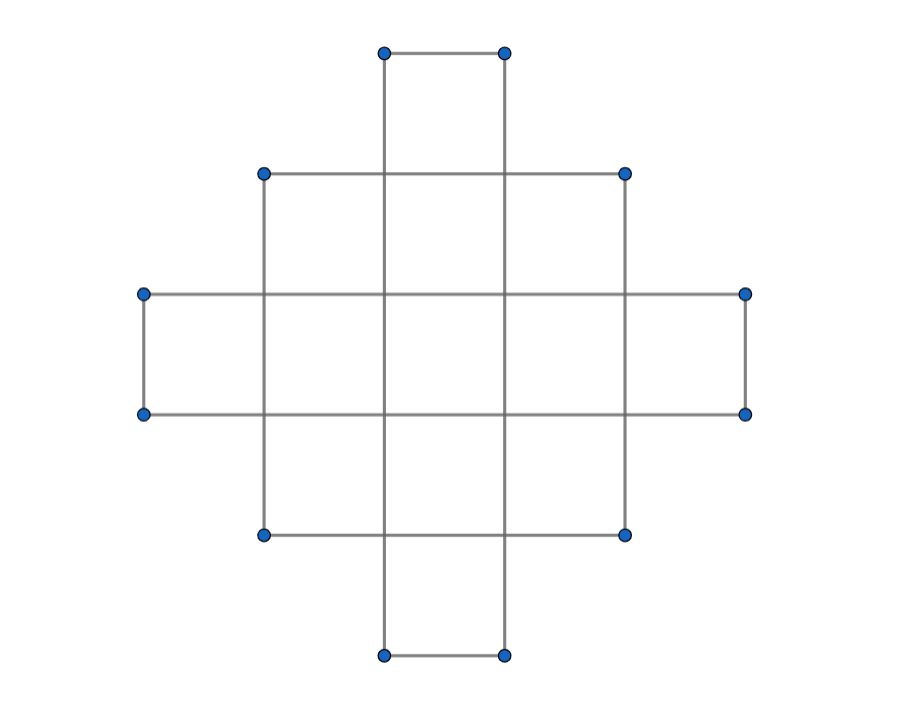
\includegraphics[scale=0.3]{Capture.png}	
	\end{center}
	You need to tile this with L-shapes made of 3 blocks. Which single blocks could you shade out of the original diagram to make this possible?


\item % Moldova, 61st Maths Olympiad (2017), 7.1 modified
Find all natural numbers $x$, $y$ and $z$ satisfying 
$$x + \frac{1}{y + \frac{1}{z}} = \frac{850862}{421}$$


\end{enumerate}


\vfill
% ASCII art
\centering
\begin{BVerbatim}
>o)
(_>
\end{BVerbatim}

\end{document}
